%% =============================================================================
%% Order-Aware Human Models for Robot Questioning and Trust
%% Target: IEEE Transactions on Cognitive and Developmental Systems (IEEEtran journal)
%% Compile: pdflatex main; bibtex main; pdflatex main; pdflatex main
%% Numbers come from ../results/*.json; figures from ../tools/make_figures.py.
%% =============================================================================
\documentclass[journal]{IEEEtran}
\usepackage{cite}
\usepackage{amsmath,amssymb,amsfonts}
\usepackage{graphicx}
\usepackage{booktabs}
\usepackage{array}
\usepackage{xcolor}
\usepackage{url}
\usepackage[hidelinks]{hyperref}
\newcommand{\fillin}[1]{{\color{red}\bfseries [FILL: #1]}}

\begin{document}
\title{Order-Aware Human Models for Robot Questioning and Trust: A Quantum-Like Model With Classical Baselines, Simulation Studies and Quantum-Circuit Execution}

\author{Yeshwanth~Guru and~Dev~Kunwar~Singh~Chauhan%
\thanks{Y. Guru and D. K. S. Chauhan are with the Department of Mechanical Engineering, Amrita School of Engineering, Amrita Vishwa Vidyapeetham, Chennai 601103, India (e-mail: g\_yeshwanth@ch.students.amrita.edu; c\_devsingh@ch.amrita.edu). Corresponding author: Yeshwanth Guru. ORCID: Y. Guru 0009-0007-6353-4033; D. K. S. Chauhan 0000-0002-1466-4567.}%
\thanks{Manuscript received \fillin{date}.}}

\markboth{IEEE Transactions on Cognitive and Developmental Systems}%
{Guru and Chauhan: Order-Aware Human Models for Robot Questioning and Trust}

\maketitle

\begin{abstract}
Robots ask people questions to resolve ambiguity, to elicit preferences and to check trust, and they treat the answers as readings of fixed beliefs. Human answers, however, depend on question order, and asking can change what a person thinks next. This paper builds an order-aware human model for robot questioning and tests it against classical alternatives. A three-dimensional quantum-like (quantum-probability) model with projector ranks is compared with an order-free Bayesian model and two anchoring models, and an open-system trust model is compared with a Markov model, in simulated populations for three robot domains: object clarification, trust and hand-over, and preference elicitation. On published data, the quantum-like model fits the Clinton--Gore order effect as well as anchoring does, whereas the Bayesian model cannot. In simulation, the quantum-like model is identified from 400 people per question order in 93\% of homogeneous data sets and is then the best predictor of answers in the unasked order, but individual differences reduce its advantage, and when people follow a classical order effect it is the worst predictor, about ten times worse than the Bayesian model. For recovering unprimed answers, randomizing question order beats model-based correction under every generator. Under open-system dynamics, a midway trust question lowers final trust by 0.076; detecting this needs about 1,600 people per condition, and a robot that always asks cannot learn it. Both models run as quantum circuits; under the noise model of a current IBM processor, answer distributions deviate by about 0.04 in total variation and the QQ equality holds to within 0.012. Quantum-like models are therefore a useful but conditional part of a robot's model of people: they should be weighted against classical models by evidence, not used alone.
\end{abstract}

\begin{IEEEkeywords}
Human--robot interaction, question order effects, quantum cognition, quantum computing, trust, user modeling.
\end{IEEEkeywords}


\section{Introduction}\label{sec:intro}
\IEEEPARstart{R}{obots} that work with people ask them questions. A service robot asks which object is meant before it grasps; a collaborative robot asks whether the person is ready before it hands over a tool; a robot that learns from feedback asks which of two trajectories is better~\cite{Christiano2017}. Help-seeking planners make asking an explicit decision: the robot acts when its plan is unambiguous and asks when it is not~\cite{Ren2023,Yuan2026}, and interactive imitation learning decides when to hand control to a person under a budget~\cite{Hoque2021}. In all of these systems the answer is treated as a reading of a fixed belief that the person already holds.

Human judgement does not behave that way. Answers depend on the order in which questions are asked: in a Gallup poll of September 1997, 50\% of respondents called Bill Clinton honest when asked about him first, but 57\% did so after a question about Al Gore, while Gore's rating fell from 68\% to 60\% in the reverse order~\cite{Moore2002}. Asking a question can also change what a person thinks next. In a motion-detection task, an intermediate judgement changed later judgements in a way that Markov models of belief change could not reproduce~\cite{Kvam2015,Busemeyer2019}. Quantum-like (quantum-probability) models represent these effects by treating a belief as a vector and a question as a projection; they predict order effects, a parameter-free regularity called the QQ equality~\cite{Wang2013b,Wang2014}, and interference between judgements~\cite{Busemeyer2012,Pothos2013a,Pothos2022}. They have been proposed for trust in automation and in human--AI teams~\cite{Roeder2023,Humr2023,Lawless2020}, but a companion systematic review found almost no tests of such models in robots or agents~\cite{Guru2026b}.

This paper asks three questions. Can a quantum-like model of a person's answers be told apart from classical alternatives with the amount of data a robot study can collect? What does a robot gain by using it, and what does it lose if the model is wrong? Does asking about trust change trust, and can the robot tell whether it does? The contributions are:
\begin{itemize}
\item an order-aware human model for robot questioning, built from a three-dimensional quantum-like question model with projector ranks, three classical baselines and two trust-dynamics models (Markov and open-system), implemented and tested in open code;
\item simulation studies in three robot domains (object clarification, trust and hand-over, preference elicitation) of model recovery, cross-order prediction and questioning design, with homogeneous and heterogeneous populations;
\item a trust study showing how a question about trust can change later trust, how many people are needed to detect it, and what error a robot makes if it ignores it;
\item a test against two published data sets (the Clinton--Gore poll and the Prisoner's Dilemma disjunction effect~\cite{Shafir1992});
\item quantum-circuit versions of both models, verified on simulators and under the noise models of current IBM quantum processors, with scripts for IBM Quantum and Amazon Braket.
\end{itemize}
Fig. \ref{fig:framework} summarizes the approach. The model also supplies a confidence signal for the learned orchestrator reviewed in a companion survey~\cite{Guru2026s3}: the predictive uncertainty about a person's answer or trust (Section \ref{sec:robot}).

\begin{figure*}[!t]
\centering
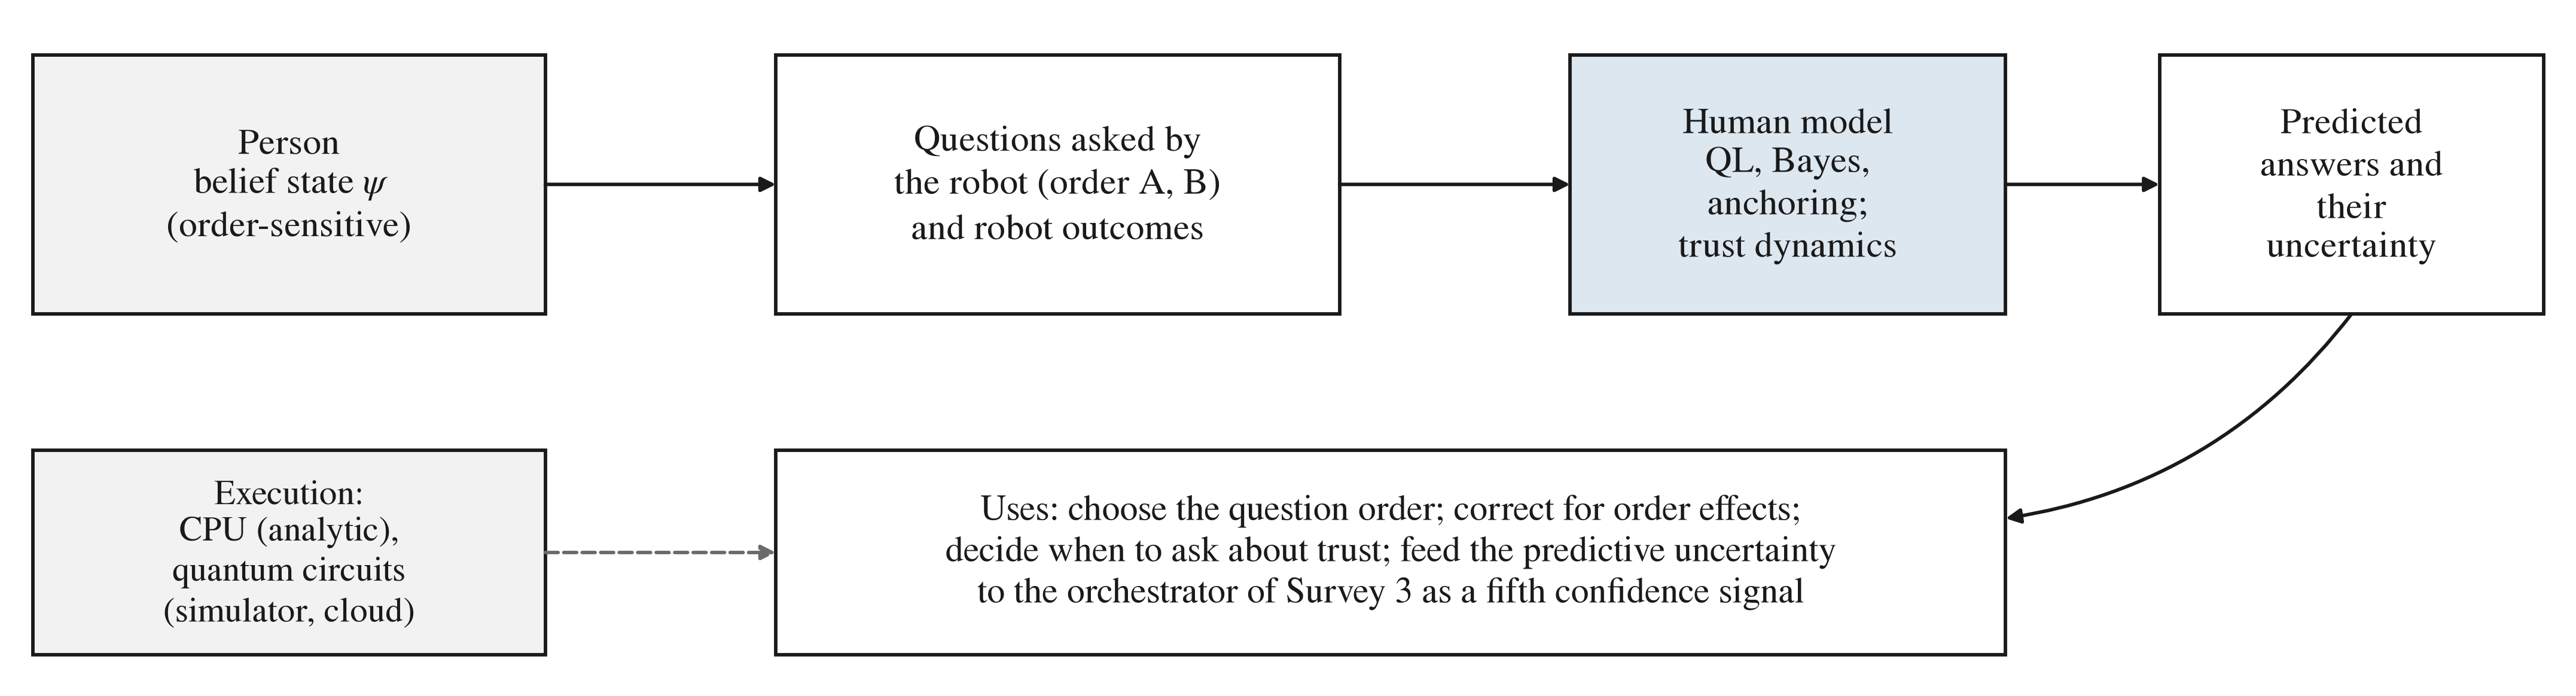
\includegraphics[width=\textwidth]{figures/Fig1_framework.png}
\caption{Approach. The robot's questions and its hand-over outcomes act on the person's belief state; competing human models (quantum-like, Bayesian, anchoring; open-system and Markov trust) predict the answers and their uncertainty, which the robot uses to choose and order its questions and passes to its orchestrator as a confidence signal. The models run analytically on a CPU or as quantum circuits.}\label{fig:framework}
\end{figure*}


\section{Background}\label{sec:background}
\subsection{Order Effects and the QQ Equality}
Let two yes/no questions $A$ and $B$ be asked in either order, and let $p_{AB}(y,n)$ be the probability of answering yes to $A$ and then no to $B$. A classical model in which answers read out a fixed joint distribution gives the same marginal probability to each question whatever its position, so it has no order effect. Order effects can be added classically, for example by letting the first answer anchor the second~\cite{Trueblood2011}. Quantum-like models predict order effects from the geometry of the questions and satisfy, for any parameters, the QQ equality
\begin{equation}
p_{AB}(y,n)+p_{AB}(n,y)=p_{BA}(y,n)+p_{BA}(n,y),\label{eq:qq}
\end{equation}
which was supported across 70 national field experiments on question order~\cite{Wang2014}. Classical models do not satisfy (\ref{eq:qq}) in general, although some do: an anchoring model with one shared weight does, and so do order-free Bayesian models trivially. Models of probability judgement with noise also produce related regularities~\cite{Costello2014,Costello2018}, and the QQ equality alone is not proof of quantum-like processing~\cite{BoyerKassem2016,Khrennikov2014,Ozawa2021}.

\subsection{Trust Dynamics}
Trust in automation grows with reliable performance and falls after failures~\cite{Lee2004}. Markov models describe trust as a probability over hidden states that is updated by outcomes; a question about trust reads the state and, averaged over the answer, leaves it unchanged. Quantum-like models of trust calibration~\cite{Roeder2023,Humr2023} and of belief change~\cite{Busemeyer2019} allow superposed states whose coherence is lost by measurement, so that asking can change what follows.


\section{Models}\label{sec:models}
\subsection{Quantum-Like Question Model}\label{sec:ql}
The person's belief is a unit vector $\psi\in\mathbb{R}^3$, and a yes answer to question $q$ is a projector $P_q$ onto either the ray of a unit vector $u_q$ (rank 1) or the plane orthogonal to it (rank 2). Answering applies the L\"uders rule~\cite{Busemeyer2012}: $p(\text{yes})=\|P_q\psi\|^2$, after which $\psi\leftarrow P_q\psi/\|P_q\psi\|$ (and the complement for no). Up to a rotation, the model has three angles,
\begin{equation}
\begin{aligned}
\psi&=e_1,\quad u_A=(\cos a,\sin a,0),\\
u_B&=(\cos b,\sin b\cos g,\sin b\sin g),
\end{aligned}
\end{equation}
plus the discrete ranks of the two yes subspaces. A two-dimensional model has only two effective parameters and cannot fit the Clinton--Gore pattern: when half the respondents answer the first question with yes, it forces the second-position rate to 0.5. The three-dimensional model with ranks (1, 2) fits it (Section \ref{sec:lit}).

\subsection{Classical Baselines}\label{sec:classical}
\textit{Bayes} is an order-free joint distribution with marginals $p_A$, $p_B$ and a correlation parameter (three parameters); response noise added to it remains in this family. \textit{Anchoring} gives the first answer at its first-position rate and pulls the second answer toward the first: $P(y_2\mid y_1)=p_2+w_q(1-p_2)$ and $P(y_2\mid n_1)=p_2(1-w_q)$ for $w_q\ge 0$ (contrast for $w_q<0$), where $q$ is the second question. With one weight (Anchoring1, three parameters) it satisfies (\ref{eq:qq}); with a weight per question (Anchoring2, four parameters) it does not. A \textit{saturated} model with a free distribution for each order (six parameters) is a reference.

\subsection{Trust Models}\label{sec:trustmodels}
A person observes a sequence of robot hand-overs with outcomes $o_t\in\{1,0\}$ (success, failure). The \textit{Markov} model has $P(\text{trust})$ initially $p_0$; after a success, distrust becomes trust with probability $s$; after a failure, trust becomes distrust with probability $f$. The \textit{open-system} model is a qubit density matrix $\rho$ with $|0\rangle$ for trust, initialized by a rotation $R_y(\phi_0)$. After a success it applies $R_y(-\alpha_s)$, after a failure $R_y(\alpha_f)$, and then dephasing of strength $\gamma$, which multiplies the off-diagonal entries by $1-\gamma$ (a Lindblad dephasing channel over one step). A trust question is a projective measurement in the trust basis. With $\gamma=1$ the model loses all coherence and behaves like a Markov chain; with $\gamma<1$ an intermediate question removes coherence that would otherwise have interfered with later rotations, so asking changes later trust.

\subsection{Robot Domains and Simulated People}\label{sec:domains}
Three domains fix a pair of questions and the size of the order effect (Fig. \ref{fig:orders}): \textit{object clarification} (``Is it the red cup?'', ``Is it the cup on the left?''), with an assimilation effect as large as in the Clinton--Gore poll; \textit{trust and hand-over} (``Do you trust the robot to hand you the tool?'', ``Was the last hand-over safe?''), with a smaller assimilation effect; and \textit{preference elicitation} (``Is trajectory 1 acceptable?'', ``Is trajectory 2 acceptable?''), with a contrast effect. For each domain, four synthetic populations generate answers: \textit{QL} (the quantum-like model fitted to the target rates); \textit{Anchoring} (the two-weight model with the same first- and second-position rates where it can reach them, so the two generators differ only in their joint structure); \textit{Bayes} (an order-free model with the QL model's A-first joint distribution); and \textit{Mixture} (half QL, half anchoring). Populations are either homogeneous or heterogeneous: in the latter, each of 2,000 simulated people draws its own parameters around the population values with a spread of 0.1 (radians for angles; logit or weight units otherwise). The target rates are illustrative choices, not estimates from people. Each simulated person answers both questions once, in one order.

\begin{figure*}[!t]
\centering
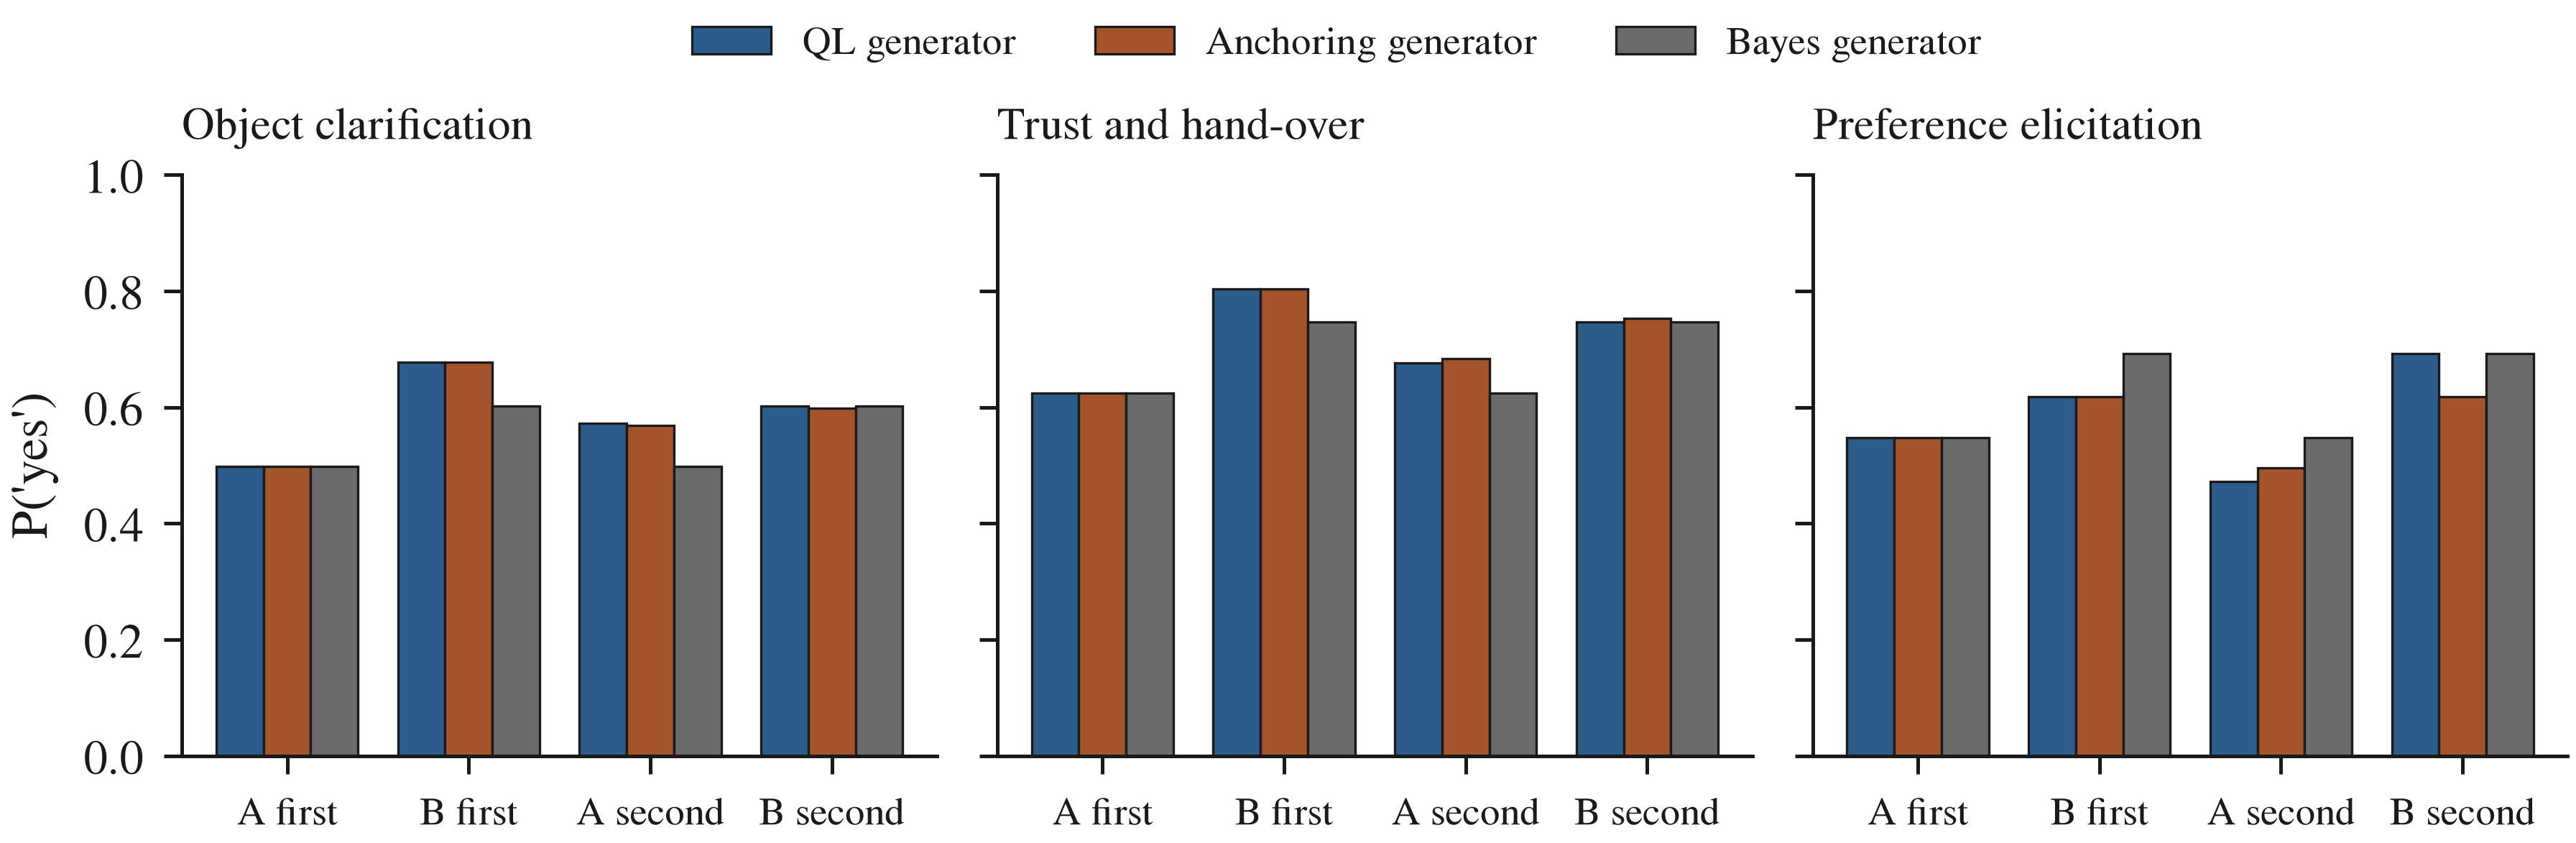
\includegraphics[width=\textwidth]{figures/Fig2_order_effects.png}
\caption{Answer rates of the synthetic populations in the three domains: probability of a yes answer to each question when it is asked first or second. QL and anchoring share these rates (except the second-position rate of B in preference elicitation, which anchoring cannot reach); Bayes has no order effect.}\label{fig:orders}
\end{figure*}


\section{Experimental Method}\label{sec:method}
\textit{Fitting and selection.} Models are fitted by maximum likelihood to answer counts (Nelder--Mead with eight random restarts; for the QL model, every rank combination). Models are compared by the Bayesian information criterion (BIC), and the QQ equality is tested with a two-sided $z$ test at $\alpha=0.05$.

\textit{Experiment 1 (model recovery).} For each domain, generator, population type and sample size (100, 400 or 1,600 people per order), answers in both orders are simulated, the QL, Bayes and Anchoring2 models are fitted, and the model with the lowest BIC is recorded; 30 repetitions per condition.

\textit{Experiment 2 (cross-order prediction).} Training data are $N$ people answering A then B ($N$ = 400 or 4,000) plus a probe of $N/10$ answering B then A. Each model predicts the B-first answer distribution; the score is the Kullback--Leibler divergence from the generator's true B-first distribution (median over 30 repetitions).

\textit{Experiment 3 (questioning design).} The robot must learn the first-position (``unprimed'') yes rates $\pi_A$ and $\pi_B$ from 400 people who each answer both questions. Designs: a fixed order AB with $\pi_B$ read from the second answers, as a robot that ignores order effects would do; a probe of 10\% or 30\% of people answering B first, with a model fitted to all answers; and a split design (half each order) using only first answers, which needs no model. With the order fixed, $\pi_B$ is not identifiable under the QL model: two parameter sets reproduce the AB answers exactly but imply different $\pi_B$ (for object clarification, 0.525 and 0.678); the probe resolves this. Score: root-mean-square error (RMSE) of $\pi_B$ over 30 repetitions.

\textit{Experiment 4 (trust).} Six hand-overs with outcomes (1, 1, 0, 1, 0, 1). In condition C0 the robot asks about trust only after the sixth hand-over; in C1 also after the third. The generators are the open-system model ($\phi_0=1.6$, $\alpha_s=0.8$, $\alpha_f=1.2$, $\gamma=0.3$; illustrative values) and the Markov model that best matches it. Both models are fitted to C0 and C1 answers with 100, 400 or 1,600 people per condition and compared by BIC. A robot that has only C1 data (it always asks midway) predicts the trust it would have found without the midway question; the RMSE of that prediction measures the cost of assuming that asking has no effect. 30 repetitions.

\textit{Experiment 5 (published data).} The models are fitted by least squares to the four Clinton--Gore rates~\cite{Moore2002,Wang2013b}; only aggregate proportions are available, so likelihoods are not computed. For the Prisoner's Dilemma~\cite{Shafir1992}, the classical law of total probability and the quantum-like law with an interference term are compared~\cite{Pothos2009}.

\textit{Experiment 6 (circuits).} The question circuits for each domain and order and the trust circuits for both conditions are run with 20,000 shots on the Qiskit Aer simulator~\cite{JavadiAbhari2024} (ideal, and with the noise models of the IBM FakeTorino and FakeBrisbane backends) and on the Amazon Braket local simulators (ideal, and with depolarizing noise of 0.5\% and 2\% after every gate). The scores are the total variation distance (TVD) between the circuit's and the analytic answer distributions and the QQ value of the circuit output.

\textit{Circuit design.} The belief space is embedded in two qubits ($e_1=|00\rangle$, $e_2=|01\rangle$, $e_3=|10\rangle$). To ask question $q$, a Householder reflection $V_q$ maps $u_q$ to $|00\rangle$; an ancilla is flipped if and only if the system is in $|00\rangle$ (a Toffoli gate between $X$ gates); only the ancilla is measured, which implements the binary L\"uders measurement without collapsing the no subspace; $V_q$ is then applied again. The trust circuit uses one qubit with $R_y$ rotations, and dephasing is applied by an ancilla that triggers a $Z$ gate with probability $\gamma/2$ and is then reset. Each circuit has a dynamic form (mid-circuit measurement and reset) and a deferred form in which every measurement is copied to a fresh ancilla and read at the end~\cite{Nielsen2010}; the latter runs on hardware without mid-circuit measurement.


\section{Results}\label{sec:results}

\subsection{Model Recovery}\label{sec:recovery}
Fig. \ref{fig:recovery} shows how often BIC selects the generating model, pooled over the three domains (90 data sets per point). In homogeneous populations, the QL generator is identified in 86\%, 93\% and 100\% of data sets with 100, 400 and 1,600 people per order; the Bayes generator in 30\%, 71\% and 98\%; and the anchoring generator in 27\%, 64\% and 97\%. Two errors dominate at small samples. With 100 people per order, data from the Bayes generator are attributed to the QL model in 63 of 90 data sets: with three parameters, the QL model absorbs sampling noise as an apparent order effect. Data from the anchoring generator are attributed to Bayes, because its order effect is small relative to sampling noise. With individual differences, recovery of the QL generator falls to 76\%, 66\% and 79\%, and in the remaining cases Bayes is selected; the average of many slightly different QL people is not itself a QL model. The QQ test rejected the equality for the anchoring generator in 31\%, 39\% and 62\% of data sets (homogeneous) and for the QL generator in at most 4\%, close to the nominal 5\%. The mixture generator was attributed to Bayes in 68--76 of 90 data sets at every sample size.

\begin{figure*}[!t]
\centering
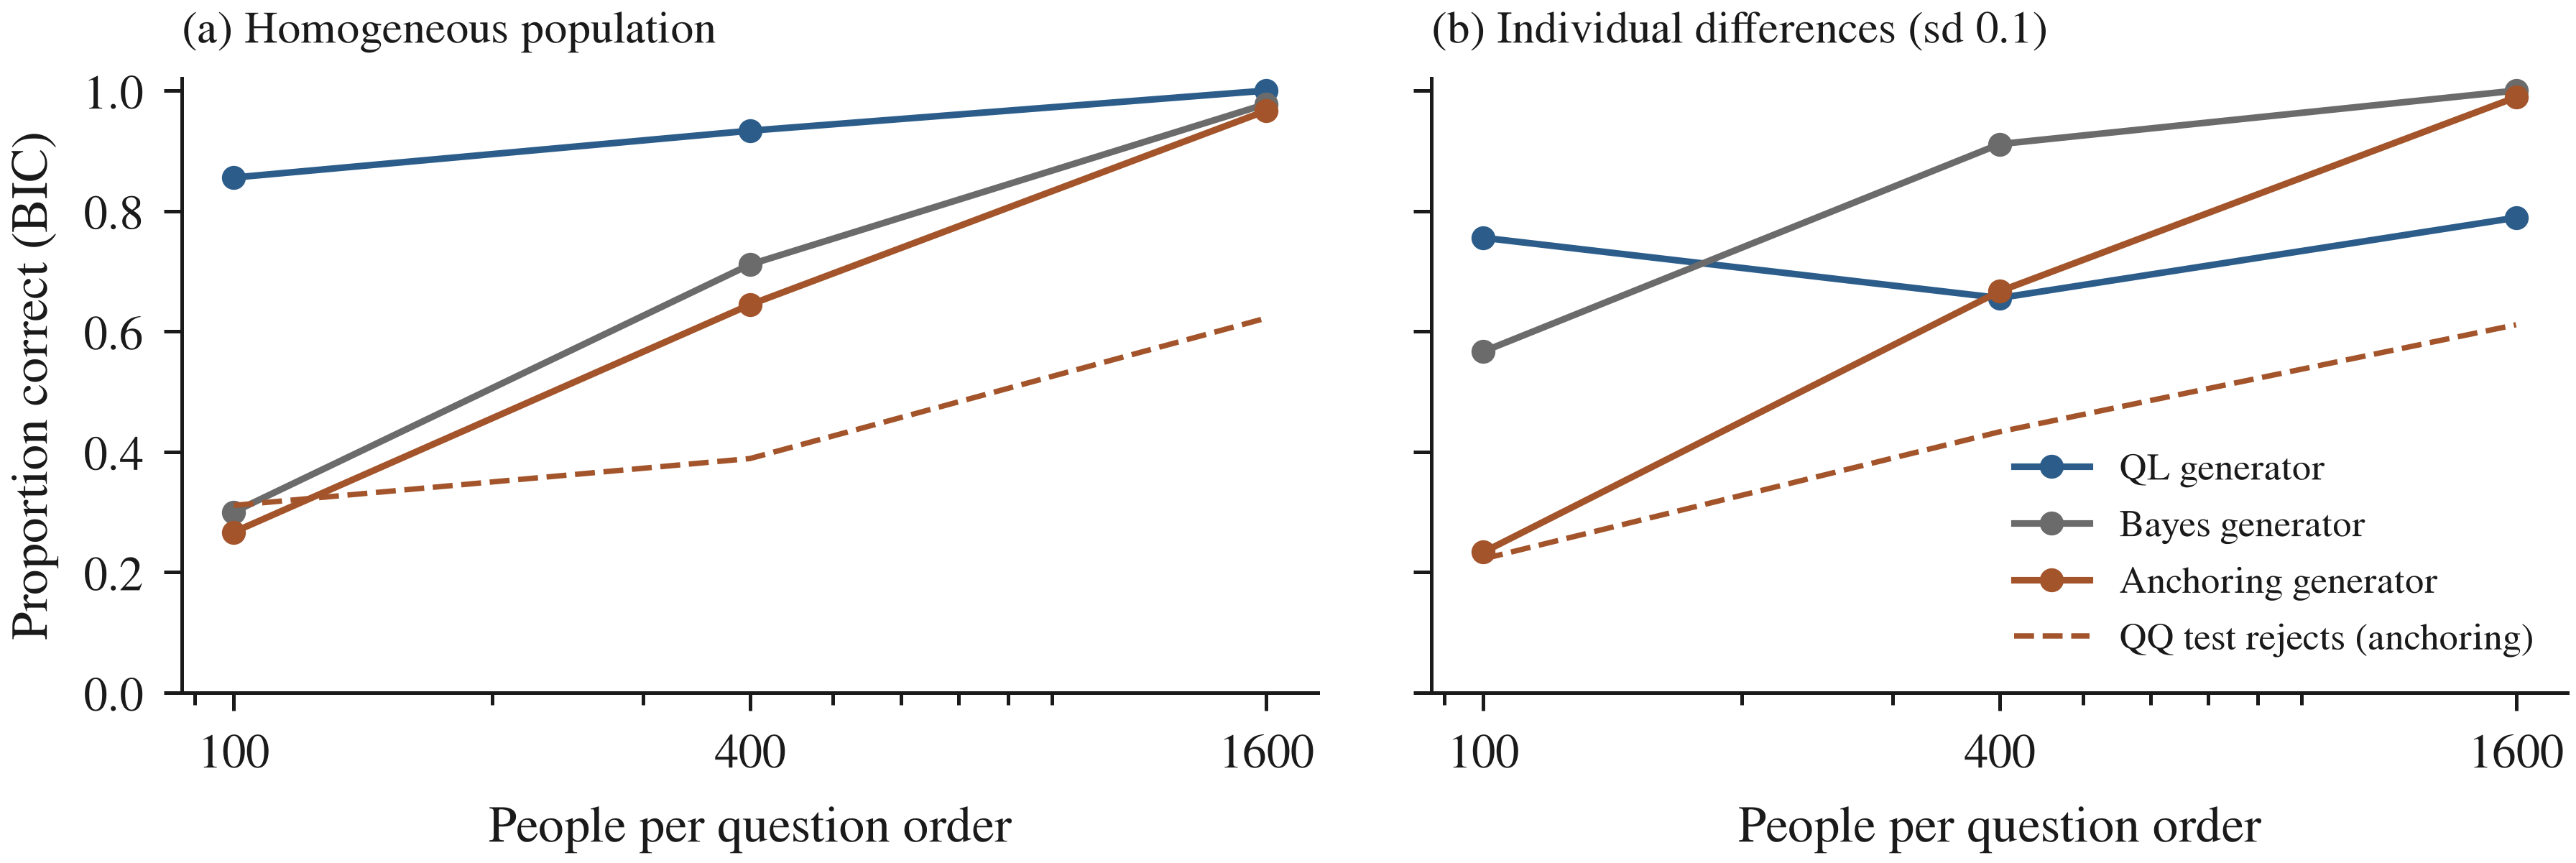
\includegraphics[width=\textwidth]{figures/Fig3_recovery.png}
\caption{Experiment 1: proportion of data sets in which BIC selects the generating model, pooled over three domains (30 repetitions each), against people per question order; dashed line, proportion of anchoring data sets in which the QQ test rejects the equality.}\label{fig:recovery}
\end{figure*}

\subsection{Cross-Order Prediction}\label{sec:crossorder}
Fig. \ref{fig:crossorder} gives the divergence between predicted and true B-first answers. When the generator is QL and the population homogeneous, the QL model predicts best (median KL 0.004 with $N=400$ and 0.0002 with $N=4{,}000$, against 0.014 and 0.011 for Bayes). With individual differences, the advantage shrinks to a tie at $N=400$ (0.013 for both) and a small margin at $N=4{,}000$ (0.007 against 0.010). When the generator is anchoring or the mixture, the QL model is the worst of all models (0.23--0.26 and 0.11--0.13), about ten times worse than Bayes, while Bayes is never worse than 0.03 under any generator. The anchoring models fail badly when the generator is QL or Bayes (0.12--0.19), because their order effect is the wrong shape.

\begin{figure*}[!t]
\centering
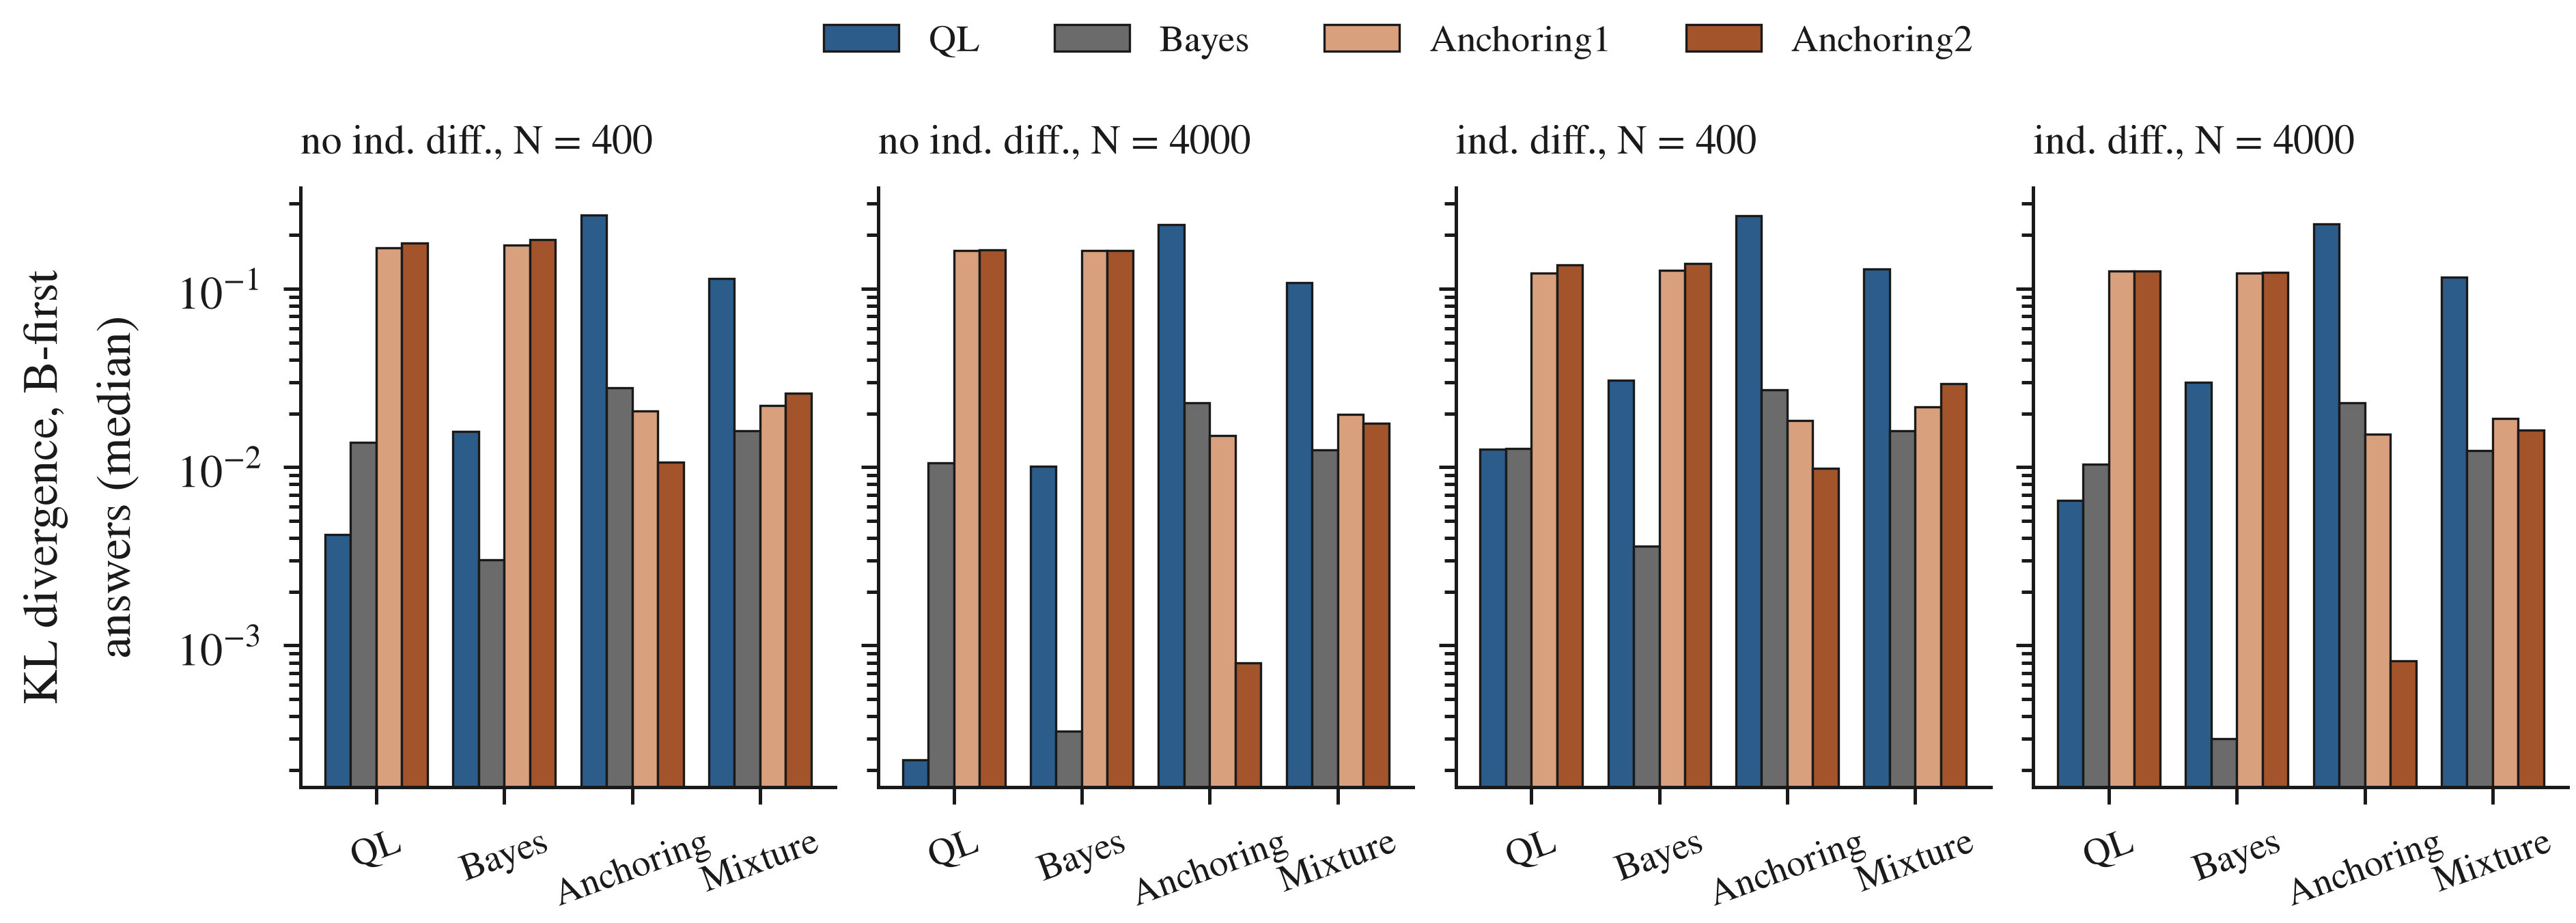
\includegraphics[width=\textwidth]{figures/Fig4_cross_order.png}
\caption{Experiment 2: Kullback--Leibler divergence between the true and the predicted B-first answer distribution (median over 30 repetitions, mean over domains, log scale), by generator, for homogeneous populations and populations with individual differences, with $N$ people answering in order AB and $N/10$ in order BA.}\label{fig:crossorder}
\end{figure*}

\subsection{Questioning Design}\label{sec:planning}
Fig. \ref{fig:planning} gives the error in the unprimed rate of the second question. The split design, which uses only first answers and no model, has an RMSE of 0.028--0.037 under every generator and population. Asking in a fixed order and reading the second answers, as a robot that ignores order effects would, gives 0.050--0.076 whenever the generator has an order effect. Model-based correction with a probe group helps only when the model is correct: with a Bayes or anchoring generator, the matching model reaches 0.021--0.030, slightly better than the split design. Under the QL generator, the QL model with a 30\% probe (0.034--0.050) does not beat the split design, because the small probe must also resolve the two-solution ambiguity of the fixed order. A wrong model is costly: the QL model applied to anchoring data gives 0.24, and the anchoring model applied to QL or Bayes data gives 0.15--0.18.

\begin{figure*}[!t]
\centering
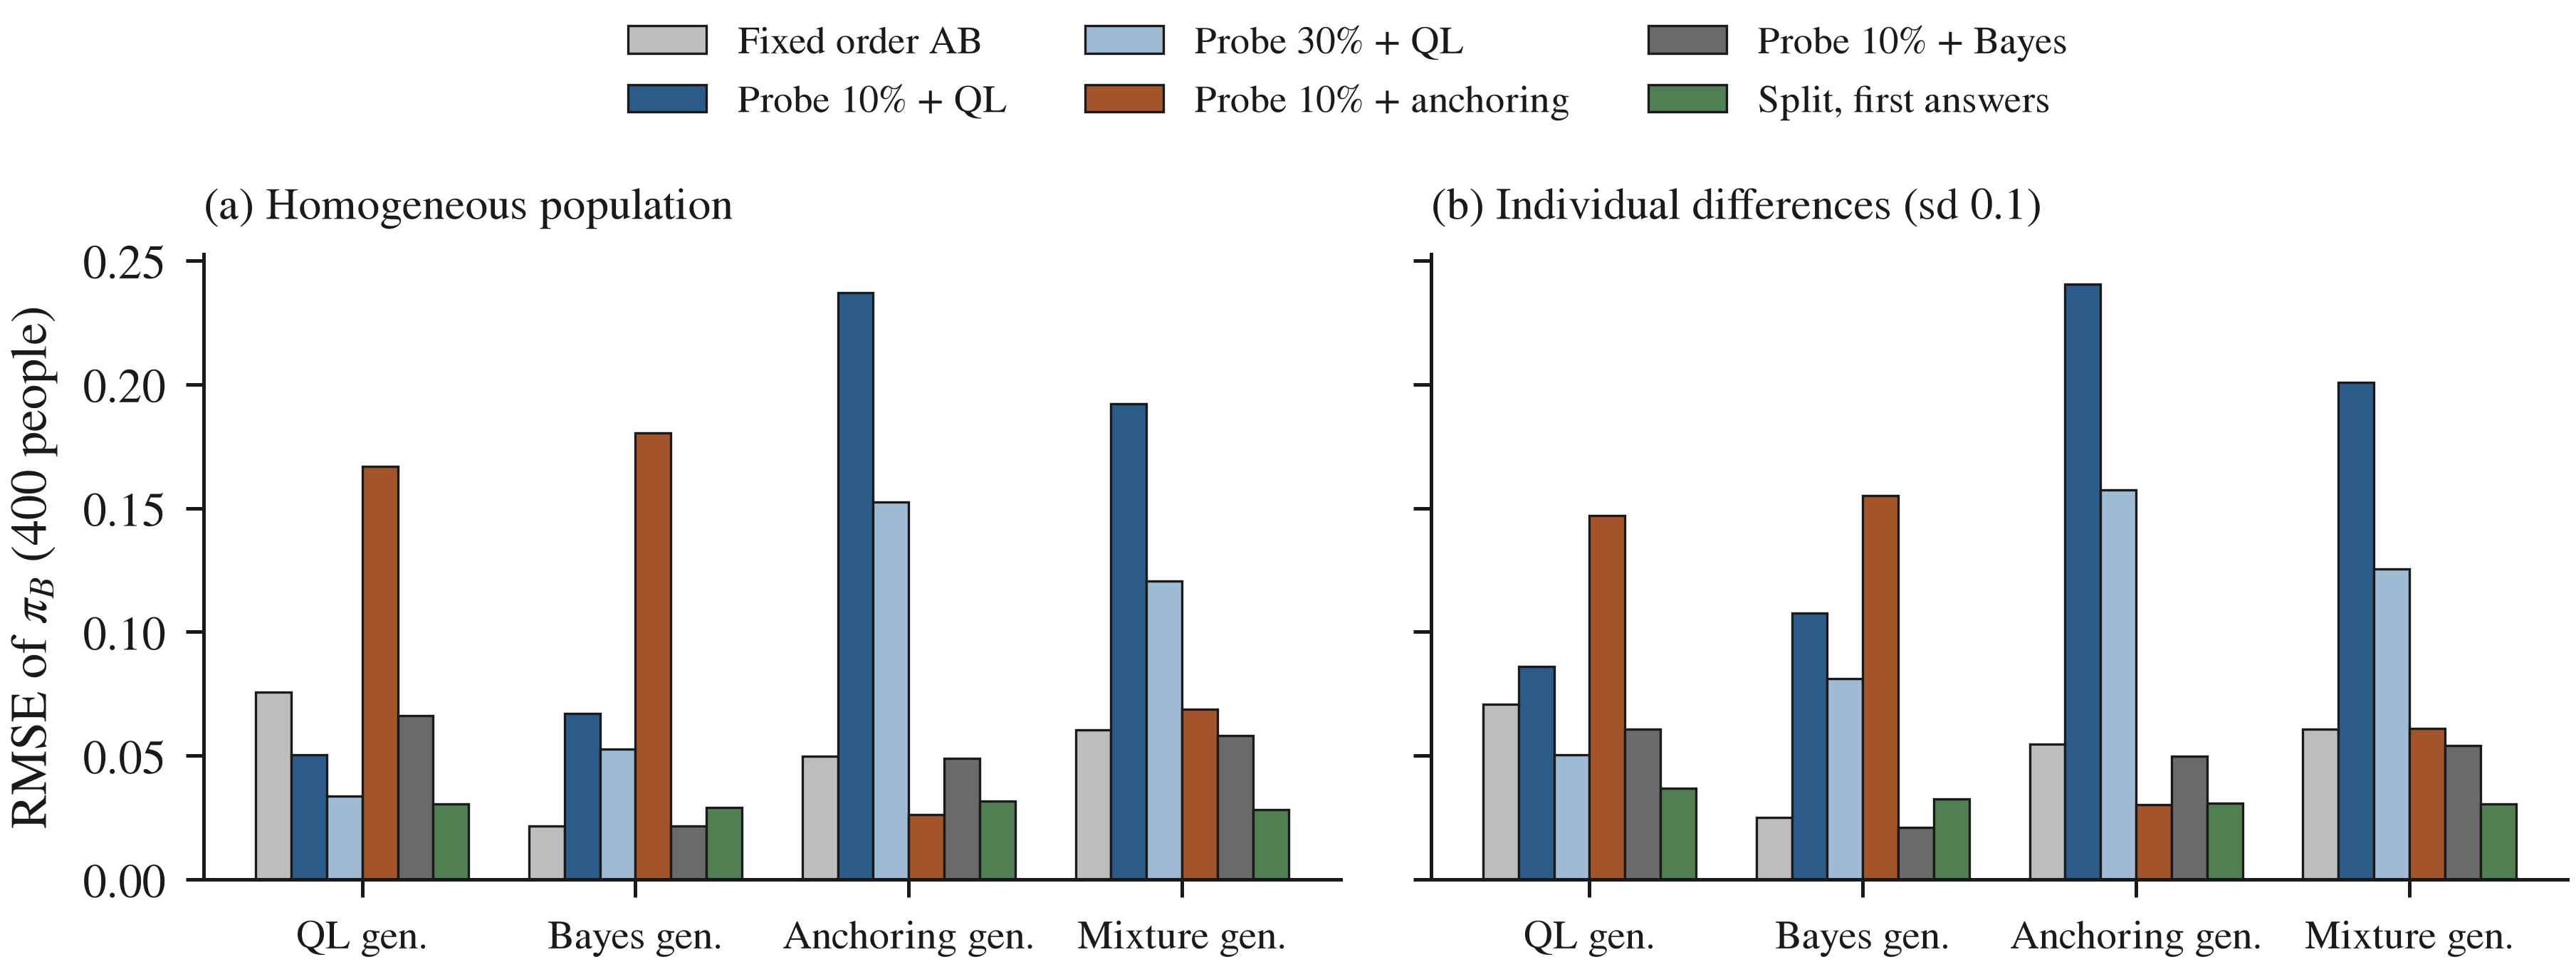
\includegraphics[width=\textwidth]{figures/Fig5_planning.png}
\caption{Experiment 3: root-mean-square error of the estimated first-position rate of question B with 400 people, by design and generator (mean over domains, 30 repetitions).}\label{fig:planning}
\end{figure*}

\subsection{Trust Dynamics}\label{sec:trust}
Under the open-system generator, the intermediate question lowers the probability of trust after the sixth hand-over from 0.725 to 0.649, a query effect of $-0.076$ (Fig. \ref{fig:trust}(a)); under the best-matching Markov model, the two conditions give the same value (0.687). BIC identifies the Markov generator in 97--100\% of data sets at all sample sizes, but identifies the open-system generator in only 3\% (100 people per condition), 27\% (400) and 93\% (1,600). A robot that always asks midway (condition C1 only) cannot learn the effect of asking: under the open-system generator, a Markov model fitted to C1 data predicts the no-question trust with a bias of $-0.06$ to $-0.08$, the size of the query effect, and the open-system model fitted to the same data is not identified (RMSE 0.15--0.17). Data from both conditions are needed.

\begin{figure*}[!t]
\centering
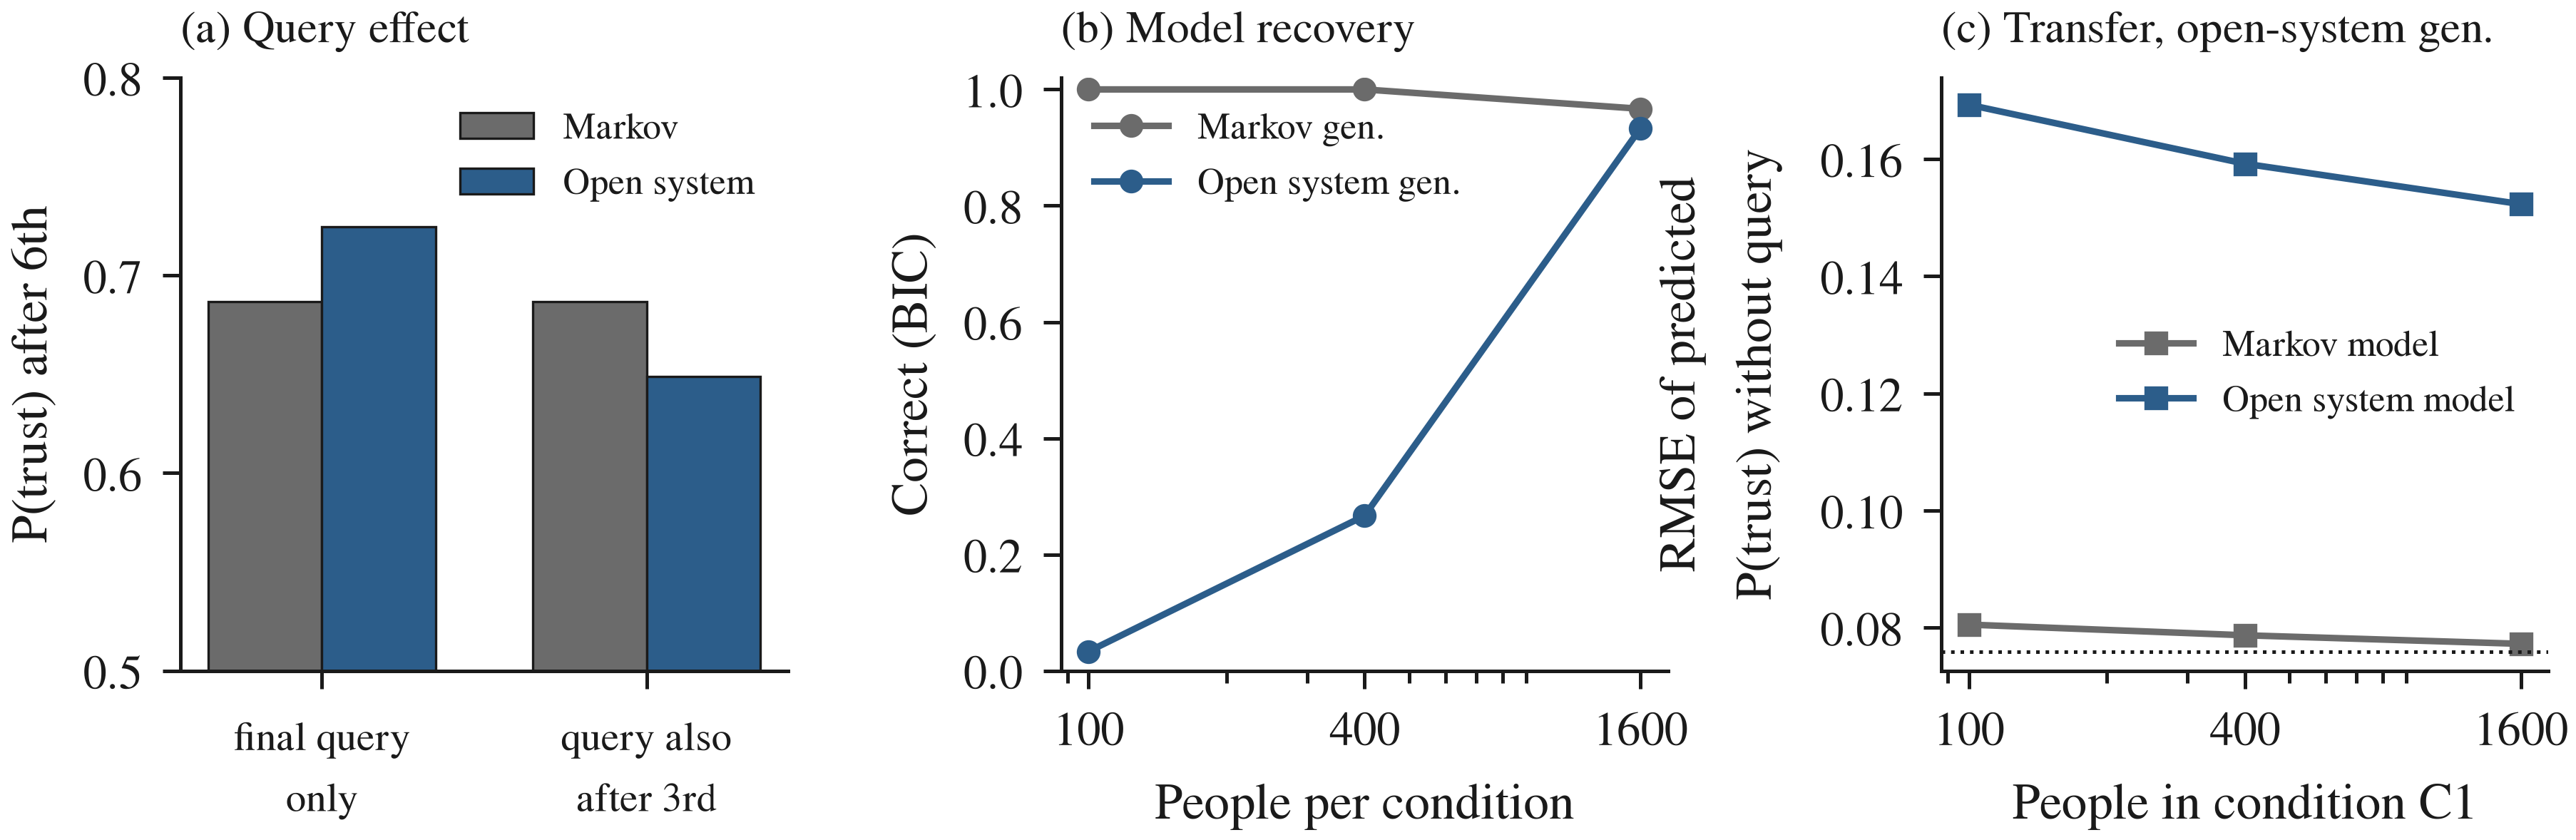
\includegraphics[width=\textwidth]{figures/Fig6_trust.png}
\caption{Experiment 4: (a) probability of trust after the sixth hand-over with and without a trust question after the third, under the open-system model and the best-matching Markov model; (b) proportion of data sets in which BIC selects the generating model; (c) error in predicting trust without the midway question from data in which it was always asked (open-system generator; dotted line, size of the query effect).}\label{fig:trust}
\end{figure*}

\subsection{Published Data}\label{sec:lit}
Table \ref{tab:lit} gives the fits to the Clinton--Gore poll. The QL model with ranks (1, 2) reproduces the four rates with a sum of squared errors of $1.4\times 10^{-5}$; the one-weight anchoring model does nearly as well ($2.5\times 10^{-5}$) and the two-weight model fits exactly, as it has as many parameters as data points. The Bayes model cannot represent an order effect ($5.7\times 10^{-3}$). The four aggregate rates therefore separate order-free from order-sensitive models but not the QL model from anchoring; the joint answer patterns, which the QQ test uses~\cite{Wang2013b,Wang2014}, are needed for that. For the Prisoner's Dilemma, the classical law of total probability requires the defection rate under uncertainty to lie between 0.84 and 0.97; the observed 0.63 lies outside. The quantum-like law reaches it with an interference phase of 1.88 rad for a belief of 0.5 that the opponent defects~\cite{Pothos2009}. One parameter is solved from one number, so this shows that the model can represent the effect, not that it predicts it.

\begin{table}[!t]
\centering
\caption{Fits to the Clinton--Gore Order Effect (Proportion Answering Yes; C Clinton, G Gore, Asked 1st or 2nd)}\label{tab:lit}
\footnotesize
\setlength{\tabcolsep}{3.5pt}
\begin{tabular}{@{}lrrrrr@{}}
\toprule
 & \textbf{C 1st} & \textbf{G 1st} & \textbf{C 2nd} & \textbf{G 2nd} & \textbf{SSE} \\ \midrule
Observed~\cite{Moore2002} & 0.50 & 0.68 & 0.57 & 0.60 & -- \\
QL (3 + ranks) & 0.498 & 0.678 & 0.572 & 0.602 & $1.4\times10^{-5}$ \\
Anchoring1 (3) & 0.498 & 0.677 & 0.573 & 0.602 & $2.5\times10^{-5}$ \\
Anchoring2 (4) & 0.500 & 0.680 & 0.570 & 0.600 & 0 \\
Bayes (3) & 0.535 & 0.640 & 0.535 & 0.640 & $5.7\times10^{-3}$ \\
\bottomrule
\end{tabular}
\end{table}

\subsection{Quantum-Circuit Execution}\label{sec:circuits}
Table \ref{tab:circ} and Fig. \ref{fig:circuits} compare circuit outputs with the analytic model. On the ideal simulators, the total variation distance is 0.003--0.007, which is shot noise at 20,000 shots, and the QQ value is within 0.004 of zero. With the noise model of the IBM FakeTorino (Heron) backend, the transpiled question circuit has depth 86--102 and 21--23 two-qubit gates; the distance rises to 0.037--0.041 in the dynamic form and 0.044--0.056 in the deferred form, and the QQ value shifts to between $-0.012$ and $-0.003$. The FakeBrisbane (Eagle) noise model gives 0.052--0.055. Depolarizing noise of 0.5\% per gate gives 0.026--0.033 and of 2\% gives 0.105--0.119, with QQ values down to $-0.039$. The trust circuit preserves the query effect under FakeTorino noise ($-0.077$ dynamic, $-0.073$ deferred, against $-0.076$ exact). No quantum hardware was used; the scripts in the repository submit the same circuits to IBM Quantum and Amazon Braket devices.

\begin{figure*}[!t]
\centering
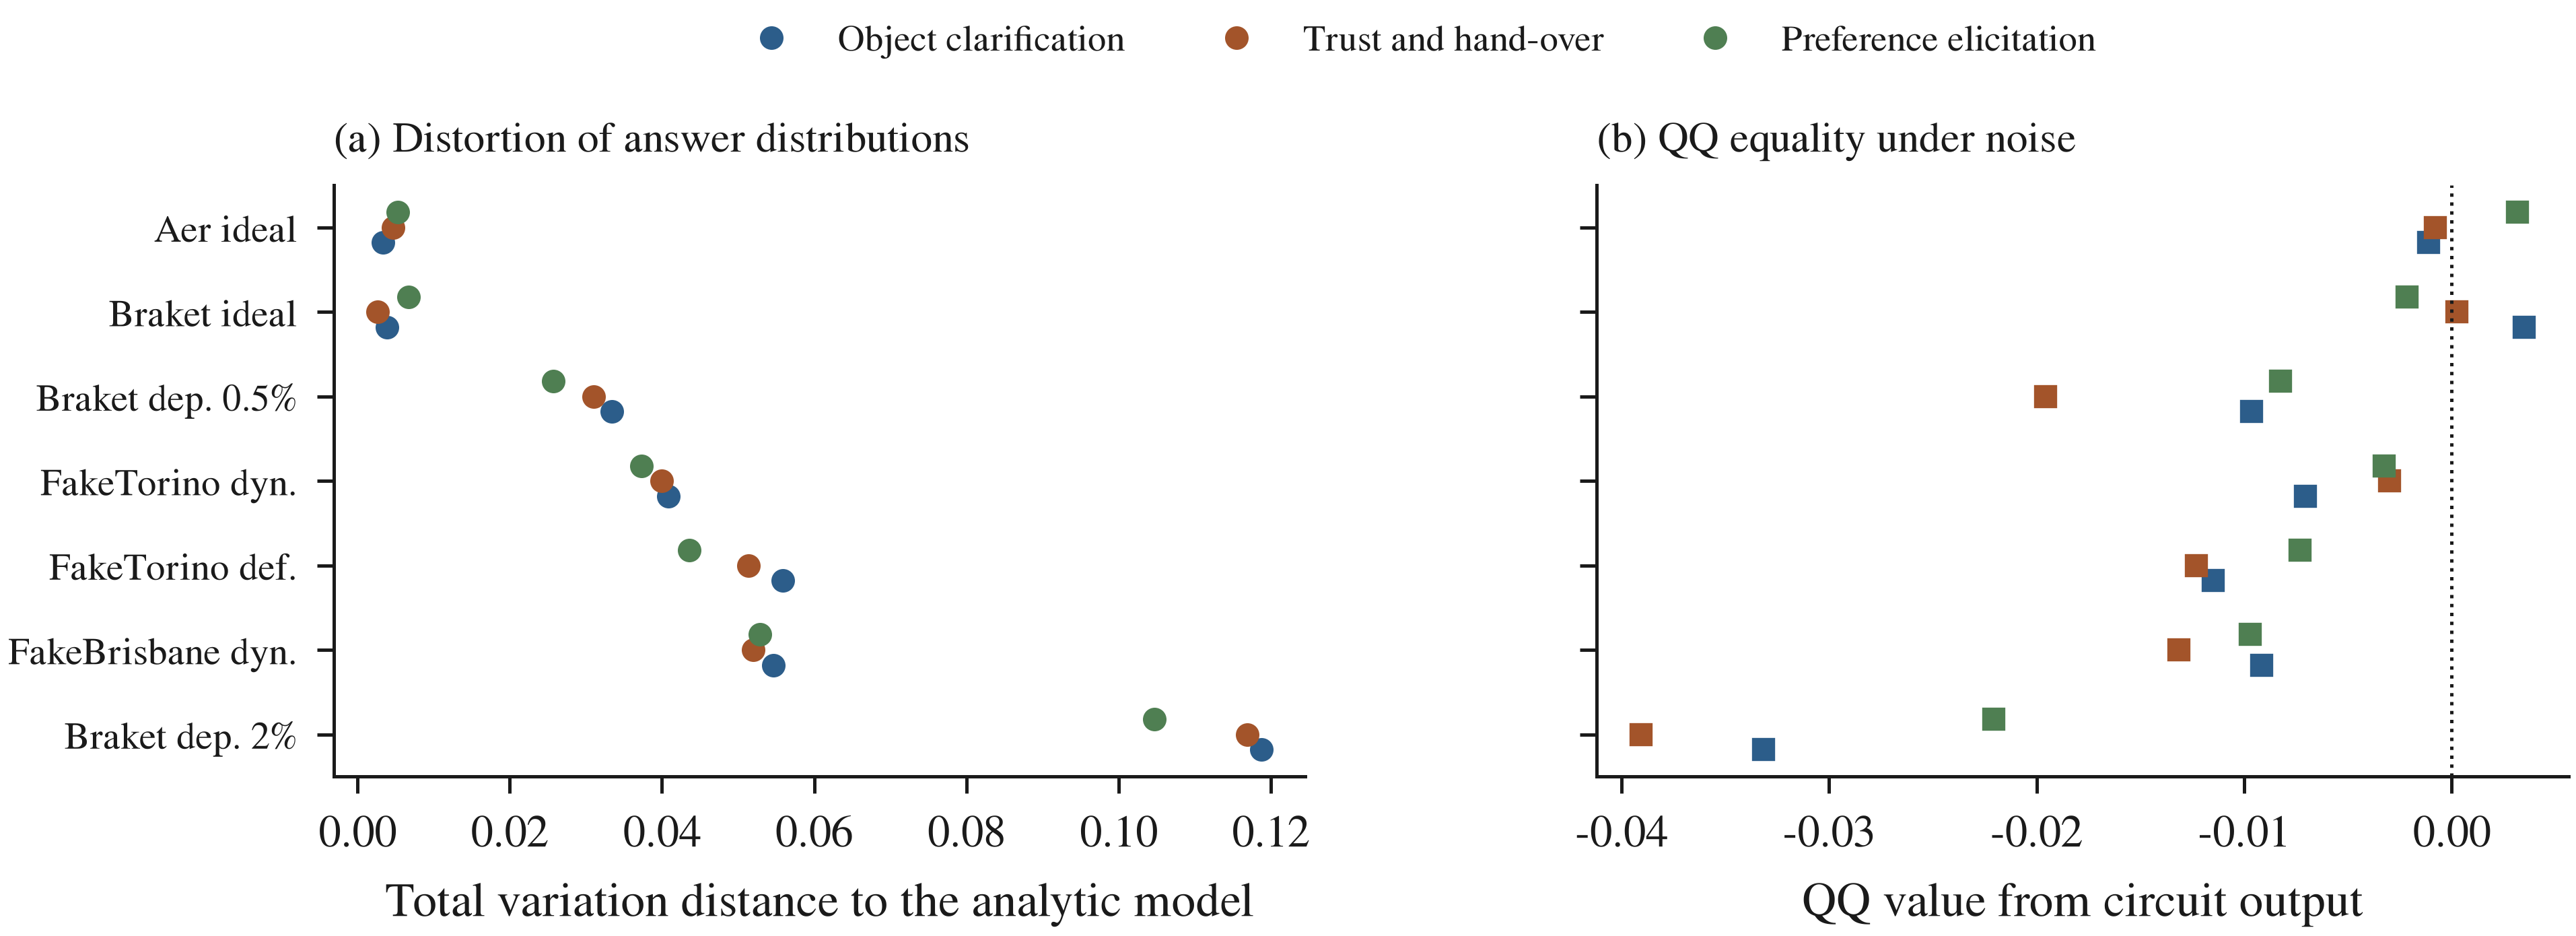
\includegraphics[width=\textwidth]{figures/Fig7_circuits.png}
\caption{Experiment 6: (a) total variation distance between the circuit output and the analytic answer distribution (mean of the two orders) and (b) QQ value of the circuit output, for each domain on ideal and noisy simulators (20,000 shots). Dyn., mid-circuit measurement; def., deferred measurement; dep., depolarizing noise per gate.}\label{fig:circuits}
\end{figure*}

\begin{table}[!t]
\centering
\caption{Question Circuits on Simulators: Range Over Three Domains (20,000 Shots)}\label{tab:circ}
\footnotesize
\begin{tabular}{@{}lll@{}}
\toprule
\textbf{Simulator} & \textbf{TVD} & \textbf{QQ value} \\ \midrule
Aer, ideal & 0.003--0.005 & $-0.001$ to 0.003 \\
Braket, ideal & 0.003--0.007 & $-0.002$ to 0.004 \\
Braket, depolarizing 0.5\% & 0.026--0.033 & $-0.020$ to $-0.008$ \\
Aer, FakeTorino, dynamic & 0.037--0.041 & $-0.007$ to $-0.003$ \\
Aer, FakeTorino, deferred & 0.044--0.056 & $-0.012$ to $-0.007$ \\
Aer, FakeBrisbane, dynamic & 0.052--0.055 & $-0.013$ to $-0.009$ \\
Braket, depolarizing 2\% & 0.105--0.119 & $-0.039$ to $-0.022$ \\
Hardware (IBM, Braket) & \multicolumn{2}{l}{\fillin{after a cloud run}} \\
\bottomrule
\end{tabular}
\end{table}


\section{Discussion}\label{sec:discussion}
\subsection{What the Quantum-Like Model Adds, and When}
The simulations give a consistent picture. The quantum-like model is the right tool when people really follow it and are similar to one another: it is then recovered reliably from a few hundred people per order and predicts the unasked order far better than the classical models. Its distinctive prediction, the QQ equality, was rejected in QL data no more often than the nominal 5\%, and it held in every circuit run to within the hardware noise. Outside these conditions the model is a liability. With small samples it reads noise as order effects; with individual differences its advantage shrinks or vanishes; and when the people follow a classical order effect, its predictions are the worst of all models. The Bayesian model, which ignores order, is never the best when order effects exist but is never far off. For a robot, this asymmetry matters more than average accuracy.

\subsection{Recommendations for Robots That Ask Questions}
Three recommendations follow. First, when the robot needs people's unprimed answers, it should randomize the order of its questions and use first answers, not correct fixed-order answers with a model; the split design was the most accurate or close to it under every generator. Second, the robot should not commit to one model of order effects. It can carry the QL, Bayes and anchoring models together, weight them by their evidence as data accumulate, and use the QQ test as a check; Experiment 1 shows that several hundred answers per order are needed before the weights become decisive. Third, asking about trust is an action, not a free reading. If trust follows open-system dynamics, a midway question lowered later trust by 0.076 in the simulation, and a robot that always asks cannot learn this effect: it must sometimes not ask. This links to help-seeking in robot planning~\cite{Ren2023,Yuan2026}, where asking is currently treated as cost-free apart from the person's time.

\subsection{Connection to Learned Orchestration}\label{sec:robot}
The companion survey frames an edge robot's controller as a meta-learned orchestrator that routes between learning modalities on calibrated confidence signals~\cite{Guru2026s3}. The human model supplies one more signal: the predictive uncertainty about the person's next answer or level of trust. The results set two conditions for using it. The signal must come from a set of models weighted by evidence, not from the QL model alone, and it must be calibrated against outcomes like the other signals, because a wrong human model is confidently wrong. The trust result adds a cost to the orchestrator's help-seeking action.

\subsection{Quantum Hardware}
The analytic models run in microseconds on a single-board computer; quantum hardware is not needed to use them. The circuits show that the representation transfers to quantum processors, and that current noise levels distort the answer distributions by about 0.04 in total variation, which is small compared with order effects of 0.07--0.08, but large compared with some QQ deviations of interest. The dynamic form is more accurate than the deferred form on the same noise model. Whether quantum hardware offers any advantage for such models, for example by evaluating many candidate human models in superposition, is an open question that this study does not address.

\subsection{Limitations}
All results except Experiment 5 come from simulated people whose parameters are illustrative, not estimated from human-robot interaction data. The models are fitted to aggregate counts, as in the survey literature; individual-level and hierarchical fitting may reduce the cost of individual differences. Only two questions are modelled, and response replicability, which standard projective models do not reproduce together with order effects~\cite{Khrennikov2014,Ozawa2021}, is not tested. The trust model has illustrative parameters and a single outcome sequence. No quantum hardware results are reported.


\section{Conclusion}\label{sec:conclusion}
This paper built and tested an order-aware model of how people answer a robot's questions and how their trust evolves when the robot asks about it. The quantum-like model reproduces published order effects as well as a classical anchoring model does and better than an order-free Bayesian model. In simulation, it can be identified and is the best predictor when people follow it and are similar to one another, but it is the worst predictor when they do not, and individual differences erode its advantage. The open-system trust model predicts that asking about trust lowers later trust, an effect that a Markov model cannot represent, that needs about 1,600 people per condition to detect, and that a robot cannot learn if it always asks. Both models run as quantum circuits and survive current hardware noise models with a total variation error of about 0.04.

The final conclusion is that quantum-like models are a useful but conditional component of a robot's model of people. They add a structure that classical models lack, and they can be tested with modest studies, but they should be used inside a set of competing models weighted by evidence, not on their own, and a robot should randomize its question order rather than correct for order effects with any single model. Whether real people interacting with real robots follow these models is the decisive open question; the pre-registered human study outlined in the repository would answer it.


\section*{Data and Code Availability}
All code, simulation results and figure scripts are in the project repository (folder \texttt{model}) and will be archived on Zenodo \fillin{Zenodo DOI}. The only human data used are the published aggregate proportions cited in Section \ref{sec:lit}.

\section*{Acknowledgment}
\fillin{acknowledgments and funding, or delete this section}

\bibliographystyle{IEEEtran}
\bibliography{refs}

\begin{IEEEbiographynophoto}{Yeshwanth Guru}
\fillin{biography}
\end{IEEEbiographynophoto}

\begin{IEEEbiographynophoto}{Dev Kunwar Singh Chauhan}
\fillin{biography}
\end{IEEEbiographynophoto}
\end{document}
